

\tikzset{every picture/.style={line width=0.75pt}} %set default line width to 0.75pt        

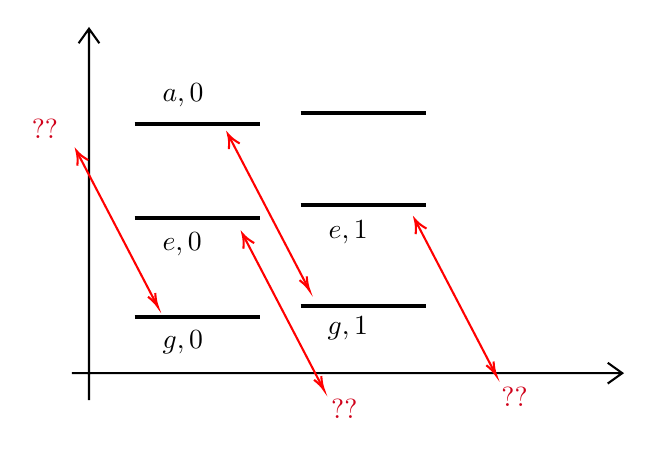
\begin{tikzpicture}[x=0.75pt,y=0.75pt,yscale=-1,xscale=1]
%uncomment if require: \path (0,199); %set diagram left start at 0, and has height of 199

%Shape: Axis 2D [id:dp7044047881463993] 
\draw  (22.83,170.89) -- (287.97,170.89)(31.04,4.94) -- (31.04,183.93) (280.97,165.89) -- (287.97,170.89) -- (280.97,175.89) (26.04,11.94) -- (31.04,4.94) -- (36.04,11.94)  ;
%Straight Lines [id:da8544066902130162] 
\draw [line width=1.5]    (53,144) -- (113.47,144) ;
%Straight Lines [id:da7205922197236949] 
\draw [line width=1.5]    (53,51) -- (113.47,51) ;
%Straight Lines [id:da5372911334007633] 
\draw [line width=1.5]    (133,138.5) -- (193.47,138.5) ;
%Straight Lines [id:da025883166300928573] 
\draw [line width=1.5]    (133,45.5) -- (193.47,45.5) ;
%Straight Lines [id:da8336819480921466] 
\draw [color={rgb, 255:red, 255; green, 0; blue, 0 }  ,draw opacity=1 ]   (98.93,57.54) -- (136.33,129.23) ;
\draw [shift={(137.26,131)}, rotate = 242.44] [color={rgb, 255:red, 255; green, 0; blue, 0 }  ,draw opacity=1 ][line width=0.75]    (6.56,-1.97) .. controls (4.17,-0.84) and (1.99,-0.18) .. (0,0) .. controls (1.99,0.18) and (4.17,0.84) .. (6.56,1.97)   ;
\draw [shift={(98,55.77)}, rotate = 62.44] [color={rgb, 255:red, 255; green, 0; blue, 0 }  ,draw opacity=1 ][line width=0.75]    (6.56,-2.94) .. controls (4.17,-1.38) and (1.99,-0.4) .. (0,0) .. controls (1.99,0.4) and (4.17,1.38) .. (6.56,2.94)   ;
%Straight Lines [id:da8918814843361473] 
\draw [color={rgb, 255:red, 255; green, 0; blue, 0 }  ,draw opacity=1 ]   (25.93,65.54) -- (63.33,137.23) ;
\draw [shift={(64.26,139)}, rotate = 242.44] [color={rgb, 255:red, 255; green, 0; blue, 0 }  ,draw opacity=1 ][line width=0.75]    (6.56,-1.97) .. controls (4.17,-0.84) and (1.99,-0.18) .. (0,0) .. controls (1.99,0.18) and (4.17,0.84) .. (6.56,1.97)   ;
\draw [shift={(25,63.77)}, rotate = 62.44] [color={rgb, 255:red, 255; green, 0; blue, 0 }  ,draw opacity=1 ][line width=0.75]    (6.56,-2.94) .. controls (4.17,-1.38) and (1.99,-0.4) .. (0,0) .. controls (1.99,0.4) and (4.17,1.38) .. (6.56,2.94)   ;
%Straight Lines [id:da2473095698421811] 
\draw [color={rgb, 255:red, 255; green, 0; blue, 0 }  ,draw opacity=1 ]   (188.93,98.54) -- (226.33,170.23) ;
\draw [shift={(227.26,172)}, rotate = 242.44] [color={rgb, 255:red, 255; green, 0; blue, 0 }  ,draw opacity=1 ][line width=0.75]    (6.56,-1.97) .. controls (4.17,-0.84) and (1.99,-0.18) .. (0,0) .. controls (1.99,0.18) and (4.17,0.84) .. (6.56,1.97)   ;
\draw [shift={(188,96.77)}, rotate = 62.44] [color={rgb, 255:red, 255; green, 0; blue, 0 }  ,draw opacity=1 ][line width=0.75]    (6.56,-2.94) .. controls (4.17,-1.38) and (1.99,-0.4) .. (0,0) .. controls (1.99,0.4) and (4.17,1.38) .. (6.56,2.94)   ;
%Straight Lines [id:da5354722999998263] 
\draw [line width=1.5]    (53,96) -- (113.47,96) ;
%Straight Lines [id:da15509678461862553] 
\draw [line width=1.5]    (133,90) -- (193.47,90) ;
%Straight Lines [id:da5426262796400413] 
\draw [color={rgb, 255:red, 255; green, 0; blue, 0 }  ,draw opacity=1 ]   (105.93,105.54) -- (143.33,177.23) ;
\draw [shift={(144.26,179)}, rotate = 242.44] [color={rgb, 255:red, 255; green, 0; blue, 0 }  ,draw opacity=1 ][line width=0.75]    (6.56,-1.97) .. controls (4.17,-0.84) and (1.99,-0.18) .. (0,0) .. controls (1.99,0.18) and (4.17,0.84) .. (6.56,1.97)   ;
\draw [shift={(105,103.77)}, rotate = 62.44] [color={rgb, 255:red, 255; green, 0; blue, 0 }  ,draw opacity=1 ][line width=0.75]    (6.56,-2.94) .. controls (4.17,-1.38) and (1.99,-0.4) .. (0,0) .. controls (1.99,0.4) and (4.17,1.38) .. (6.56,2.94)   ;

% Text Node
\draw (65,148.9) node [anchor=north west][inner sep=0.75pt]    {$\ket{g,0}$};
% Text Node
\draw (145,95.9) node [anchor=north west][inner sep=0.75pt]    {$\ket{e,1}$};
% Text Node
\draw (144.5,142.4) node [anchor=north west][inner sep=0.75pt]    {$\ket{g,1}$};
% Text Node
\draw (2,47) node [anchor=north west][inner sep=0.75pt]  [color={rgb, 255:red, 208; green, 2; blue, 27 }  ,opacity=1 ] [align=left] {??};
% Text Node
\draw (65,101.9) node [anchor=north west][inner sep=0.75pt]    {$\ket{e,0}$};
\draw (65,30) node [anchor=north west][inner sep=0.75pt]    {$\ket{a,0}$};
% Text Node
\draw (146.26,182) node [anchor=north west][inner sep=0.75pt]  [color={rgb, 255:red, 208; green, 2; blue, 27 }  ,opacity=1 ] [align=left] {??};
% Text Node
\draw (228.26,176) node [anchor=north west][inner sep=0.75pt]  [color={rgb, 255:red, 208; green, 2; blue, 27 }  ,opacity=1 ] [align=left] {??};


\end{tikzpicture}
